\documentclass[runningheads]{llncs}
\pdfinfo{/Author () /Title () /Subject () /Keywords ()}

\usepackage[T1]{fontenc}
\usepackage{lmodern}
\usepackage{graphicx}
\usepackage{amsmath,amssymb}
\usepackage{booktabs}
\usepackage{multirow}
\usepackage[hyphens]{url}
\Urlmuskip=0mu plus 2mu\relax
\usepackage{cite}
\usepackage[expansion=false]{microtype}

\sloppy
\emergencystretch=3em

\begin{document}

\title{SCHR-Bench: Evaluating Security-Critical Hallucinations in LLM-Assisted Binary Reverse Engineering via Ground-Truth Mutations}

\titlerunning{SCHR-Bench: Evaluating Security-Critical Hallucinations in SRE}

\author{Anonymous}
\authorrunning{Anonymous}
\institute{Anonymous}

\maketitle

\begin{abstract}
Large Language Models (LLMs) are increasingly integrated into software reverse engineering (SRE) workflows to summarize stripped pseudocode and assist analysts in reasoning about binary behavior. However, recent empirical studies reveal that state-of-the-art LLMs struggle with fine-grained semantic logic in stripped binaries: Pordanesh and Tan~\cite{pordanesh2024exploring} reported substantial analyst errors on stealth and persistence routines across decompiled samples ($n=15$), while human--LLM teaming experiments by Basque et al.~\cite{basque2026decompiling} (NDSS 2026) revealed that automated hallucinations severely degrade comprehension workflows on custom algorithms ($\ge 231\%$ slowdown). Classical surface metrics such as BLEU measure lexical form rather than whether an LLM detects semantics-inverting code changes. In this paper, we present \textbf{SCHR-Bench}, a controlled differential mutation benchmark evaluating \textbf{Security-Critical Hallucination Rates (SCHR)} on decompiler-style pseudocode using 40 paired security-decision functions ($N = 80$ compiled PE64 variants across five functional families) with execution-verified ground truth (160 assertions in Experiment E0). Across \textbf{1,020 logged evaluations} ($\tau = 0.0, \text{seed} = 42$) spanning Layer 1 (return-value execution oracle) and Layer 2 (paired multiple-choice gold set) across Context Tiers CT1--CT3, we evaluate \texttt{LLaMA-3.1 8B} and \texttt{Qwen2.5-Coder 14B}. Our findings reveal that: (1) under stripped pseudocode (CT1), models exhibit substantial SCHR ($38.8\%$ on LLaMA-3.1, $23.8\%$ on Qwen2.5-Coder), with pair-level accuracy (correct on both original and mutant) dropping to $25.0\%$ and $57.5\%$; (2) when models err on mutants, up to $100\%$ of failures reproduce the unmutated baseline return value (canonical parroting); (3) pairs with SCHR errors exhibit significantly higher pairwise explanation similarity ($\text{BLEU} \in [0.423, 0.584]$) than error-free pairs ($\text{BLEU} \in [0.191, 0.334]$, $\rho \in [+0.124, +0.495]$), providing an exploratory post-hoc screening signal (AUROC up to $0.800$ on LLaMA and $0.811$ on Qwen); and (4) passive context escalation to raw assembly (CT2) and callee specifications (CT3) yields no statistically significant error reduction under McNemar's paired test ($p \in [0.3588, 1.0000]$).

\keywords{Reverse Engineering \and Large Language Models \and Hallucination Evaluation \and Differential Mutation Testing \and Stripped Pseudocode \and Code Obfuscation.}
\end{abstract}

\section{Introduction}
Software Reverse Engineering (SRE) of stripped binary executables is an essential capability in security auditing, vulnerability assessment, and incident response~\cite{shoshitaishvili2016sok,cifuentes1995decompilation}. Because raw assembly instructions impose heavy cognitive load on analysts, operational workflows rely on decompilers such as NSA Ghidra~\cite{ghidra2024nsa} to lift machine code into C-like pseudocode~\cite{yakdan2015norepdb}. Recently, Large Language Models (LLMs) have been widely adopted to summarize decompiled functions, infer variable roles, and explain branch conditions~\cite{pordanesh2024exploring,basque2026decompiling,tan2024llm4decompile,hui2024qwen25coder,dubey2024llama3}.

However, LLMs remain prone to plausible-sounding \textit{hallucinations}~\cite{ji2023hallucination,min2023factscore}. Empirical evidence highlights the operational severity of this problem in software reverse engineering: in an exploratory study of GPT-4 on decompiled malware subroutines, Pordanesh and Tan~\cite{pordanesh2024exploring} (Table~III, Questions~7--8) observed substantial failure rates on security-critical logic, failing on $46.7\%$ ($7/15$) of stealth techniques and $26.7\%$ ($4/15$) of persistence mechanisms across $n=15$ decompiled samples. Furthermore, in an extensive human-subject study tracking 48 reverse engineers across 109 hours, Basque et al.~\cite{basque2026decompiling} (NDSS 2026) demonstrated that while LLM assistance can accelerate standard library triage, analysts required at least $231\%$ more time on custom algorithms, and unverified vulnerability hallucinations actively degraded analyst comprehension scores by leading practitioners down false diagnostic paths. Similarly, Katpara and Sankaran~\cite{katpara2026firmware} identified the absence of hallucination-specific benchmarks for binary logic as an urgent open research gap.

\textbf{Scope and Benchmarking Strategy:} To construct a reproducible benchmark with deterministic ground truth without executing live malware, requiring commercial IDA Pro licenses, or relying on subjective manual labeling from scratch, we scope \textbf{SCHR-Bench} to x86-64 Windows PE functions under static analysis (NSA Ghidra~\cite{ghidra2024nsa} and GNU \texttt{objdump}) and light-to-moderate structural transformations. While commercial virtualization packers (e.g., VMProtect) destroy decompiler control-flow recovery, SCHR-Bench targets the core dilemma of neural decompilation: measuring whether an LLM notices when a single security-flavored branch condition, cryptographic constant, or state-update operation has been inverted or altered ($f_{\text{orig}}$ vs.\ $f_{\text{mut}}$), and investigating whether pairwise explanation similarity (BLEU) across differential pairs can serve as an exploratory screening signal for semantic inertia in regression-testing workflows.

\begin{figure}[t]
\centering
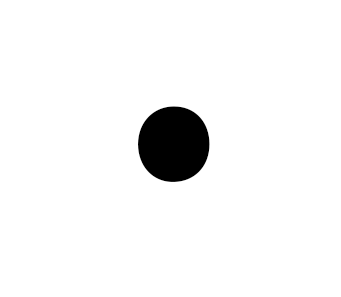
\includegraphics[width=0.96\textwidth]{figures/fig1.png}
\caption{Overview of the SCHR-Bench Evaluation Pipeline: (1) Tier 1 Host GPU Inference Server running Ollama (\texttt{llama3.1:8b} and \texttt{qwen2.5-coder:14b} at $\tau = 0.0, \text{seed} = 42$); and (2) Tier 2 Compilation, Context Generation, and Evaluation Rig executing MinGW-w64 compilation, context and real \texttt{objdump -d} assembly construction, and statistical evaluation. Note: Tier 3 shown in the diagram represents an optional isolated sandbox used only for qualitative grounding (Section~\ref{sec:case_study}).}
\label{fig:architecture}
\end{figure}

We investigate four research questions (RQ1--RQ4) and their corresponding hypotheses (H1--H4):
\begin{itemize}
    \item \textbf{RQ1 (Baseline Mutation Sensitivity --- H1):} When a security-critical function undergoes a single-point mutation (e.g., inverting an anti-debug branch or altering an XOR key), does the LLM detect the behavioral change or repeat the unmutated baseline answer?
    \item \textbf{RQ2 (Differential Pair Sensitivity \& Pairwise BLEU Screening --- H2):} What is the pair-level accuracy across original and mutated variants ($\text{SCHR}_{\text{orig}}$ vs.\ $\text{SCHR}_{\text{mut}}$), and can pairwise explanation similarity (1--3-gram BLEU~\cite{papineni2002bleu}) between $f_{\text{orig}}$ and $f_{\text{mut}}$ serve as an exploratory post-hoc screening signal for semantic inertia in differential regression audits?
    \item \textbf{RQ3 (Context Escalation with Assembly Anchor --- H3):} Does appending assembly listings (CT2) and constant/callee specifications (CT3) reduce SCHR compared to stripped pseudocode alone (CT1)?
    \item \textbf{RQ4 (Impact of Structural Obfuscation --- H4):} How do light-to-moderate structural obfuscation templates (\texttt{Obf0}--\texttt{Obf3}) affect SCHR in an exploratory pilot subset ($N=10$)?
\end{itemize}
All code, C sources, compiled PE64 binaries, real \texttt{objdump} disassembly, 240-item paired MCQ gold set, and 1,020 logged runs are available at \url{https://anonymous.4open.science/r/SCHR-Bench-Anon-827B}.

\section{Related Work}

\subsection{Empirical Studies of LLMs in Binary Reverse Engineering}
Table~\ref{tab:guideline_related} summarizes the five foundational studies that motivate SCHR-Bench:
\begin{enumerate}
    \item \textbf{Error Rates on Stealth and Evasion (Pordanesh \& Tan, 2024~\cite{pordanesh2024exploring}):} Demonstrated that LLMs struggle with low-level evasion logic ($7/15$ errors) and persistence ($4/15$) in decompiled samples ($n=15$), directly motivating our evaluation of localized decision semantics.
    \item \textbf{Operational Cost of Hallucinations (Basque et al., NDSS 2026~\cite{basque2026decompiling}):} Demonstrated through an empirical user study ($N=48$) that hallucinated decompilation artifacts induce workflow slowdowns on non-standard algorithms, emphasizing the necessity of formal verification over blind trust.
    \item \textbf{Adapting Mutation Testing from Hardware HDL to Binary SRE (Qayyum et al., 2025~\cite{qayyum2025verilog}):} Qayyum et al.\ applied mutation operators and multi-stage specification context to evaluate LLM bug identification in \textbf{Verilog HDL} hardware designs. Because hardware register-transfer level (RTL) mutations cannot be inherited directly for stripped x86-64 software binaries, we explicitly design and execution-verify five binary-oriented mutation operator families ($\mathcal{M}_1$--$\mathcal{M}_5$, Section 3.4) and adapt their context escalation concept into four static binary context tiers (CT1--CT4).
    \item \textbf{Atomic Claim Evaluation (Min et al., EMNLP 2023~\cite{min2023factscore}):} FActScore decomposes long-form text generation into atomic factual claims verified against a knowledge source. Rather than relying solely on subjective free-text grading, we pair each atomic mutation with an execution-verified return-value oracle and a 240-item full-factorial mutation-aware MCQ gold set.
    \item \textbf{Benchmark Gaps in Malware \& Firmware RE (Katpara \& Sankaran, 2026~\cite{katpara2026firmware}):} Surveying 118 reverse engineering studies (2014--2026), Katpara and Sankaran highlighted the absence of standardized benchmarks for quantifying LLM hallucinations on low-level binary and malware logic (Gaps 7 and 8).
\end{enumerate}

\begin{table}[t]
\caption{Summary of key related literature and how each informs the design of SCHR-Bench.}\label{tab:guideline_related}
\centering
\resizebox{0.98\textwidth}{!}{%
\begin{tabular}{@{}lll@{}}
\toprule
\textbf{Reference} & \textbf{Key Empirical Finding / Method} & \textbf{Role in SCHR-Bench Design} \\
\midrule
Pordanesh \& Tan (2024)~\cite{pordanesh2024exploring} & Reported failure rates on stealth ($7/15$) and persistence ($4/15$) across $n=15$ samples & Direct motivation for measuring SCHR on security-flavored logic \\
Basque et al.\ (NDSS 2026)~\cite{basque2026decompiling} & Controlled human study ($N=48$); $\ge 231\%$ time inflation on custom algorithms; hallucination risks & Demonstrates operational cost of undetected RE hallucinations \\
Qayyum et al.\ (TODAES 2025)~\cite{qayyum2025verilog} & Mutation testing \& tiered context for \textbf{Verilog HDL} debugging & Adapted from Verilog HDL into 5 binary mutation families ($\mathcal{M}_1$--$\mathcal{M}_5$) \& CT1--CT4 \\
Min et al.\ (EMNLP 2023)~\cite{min2023factscore} & \textbf{FActScore}: atomic claim verification of LLM generations & Foundation for atomic mutation-aware MCQ and return-value grading \\
Katpara \& Sankaran (2026)~\cite{katpara2026firmware} & Identifies \textbf{Gaps 7 \& 8}: lack of hallucination benchmarks in binary RE & Positions SCHR-Bench as a controlled ground-truth benchmark \\
\bottomrule
\end{tabular}%
}
\end{table}

\subsection{Differential Mutation Testing vs.\ Atomic Fact Verification}
Prior evaluations of LLMs in binary reverse engineering have largely focused on atomic claim verification (e.g., assessing whether isolated decompiler assertions or recovered variable types satisfy runtime execution constraints~\cite{pordanesh2024exploring,tan2024llm4decompile}). In contrast, SCHR-Bench introduces \textit{differential pair sensitivity}: rather than evaluating disconnected statements about a single binary, it subjects function pairs ($f_{\text{orig}}$ vs.\ $f_{\text{mut}}$) to single-point semantic mutations with execution-verified ground truth. This directly measures whether an LLM detects security-decision inversions or falls victim to memorized template priors.

\subsection{Decompiler Recovery and Neural Refinement}
Classic decompilers reconstruct high-level control flow from machine code~\cite{cifuentes1995decompilation,yakdan2015norepdb,schwarz2002disassembly}, while neural decompilation frameworks such as DIRE~\cite{lacomis2019dire}, DIRTY~\cite{chen2022dirty}, and VarBERT~\cite{pal2024varbert} recover identifier names and variable types, and LLM4Decompile~\cite{tan2024llm4decompile} targets re-compilable C code. In parallel, representation models such as TREX~\cite{pei2021trex} learn execution semantics from micro-traces for binary similarity, while code execution benchmarks (CRUXEval~\cite{gu2024cruxeval}, CodeMind~\cite{liu2024codemind}) evaluate execution reasoning on source code. SCHR-Bench bridges this gap by testing differential semantic sensitivity~\cite{jia2011analysis} on decompiler-style pseudocode under single-point mutations.

\section{The SCHR-Bench Framework}

\subsection{Task Formulation and Metric Definitions}
Let $f_{\text{orig}}$ and $f_{\text{mut}} = \mathcal{M}(f_{\text{orig}})$ denote a pair of original and mutated C functions with identical signature \texttt{int target(int a, int b, int c)}. Across 40 function pairs, our dataset comprises $N = 80$ individual function variants (40 original and 40 mutant units). We evaluate models across two complementary automated layers implemented in \path{code/step3_mcp_server_and_benchmark.py} and \path{code/step4_compute_statistics_and_tables.py}:
\begin{enumerate}
    \item \textbf{Layer 1 --- Concrete Return-Value \& Explanation Task (\texttt{--mode return}, 540 runs):} Given code representation $\mathcal{D}_k(i)$ ($N=80$ per tier across CT1, CT2, CT3, plus 60 E4 obfuscation pilot runs) and discriminating input vector $x_i = (a_i, b_i, c_i)$ (Vector 1 from \path{ground_truth_manifest.json}), the LLM outputs a JSON object with its predicted integer return value $\hat{y}_i \in \mathbb{Z}$ (\path{predicted_return}) and a technical explanation $\mathcal{Y}_i$ (\path{security_interpretation}).
    \item \textbf{Layer 2 --- Full-Factorial Paired Multiple-Choice Gold Set (\texttt{--mode mcq}, 480 runs):} Given $\mathcal{D}_k(i)$ (where CT2 and CT3 include real \texttt{objdump -d -M intel} disassembly from the compiled PE64 binary) and a 4-option question from \path{dataset/gold_set_mcq.json} (240 items per model = 480 total runs: all $N=80$ variants evaluated across all 3 tiers CT1, CT2, and CT3; balanced 60 A, 60 B, 60 C, 60 D, with the longest option correct in exactly 60/240 = 25.0\% of items to prevent length-cue guessing), the LLM selects option $\hat{c}_i \in \{\text{A, B, C, D}\}$.
\end{enumerate}

We define two primary error metrics:
\begin{enumerate}
    \item \textbf{Security-Critical Hallucination Rate (SCHR):} The proportion of evaluation units ($N=80$) where the model's prediction ($\hat{y}_i$ in return-value mode or $\hat{c}_i$ in MCQ mode) does not match the execution-verified ground truth ($y_i^*$ or $c_i^*$):
    \begin{equation}
    \text{SCHR} = \frac{1}{N} \sum_{i=1}^N \mathbb{I}\left( \hat{y}_i \neq y_i^* \right)
    \end{equation}
    \item \textbf{Mutant Miss Rate:} Across the $N_{\text{mut}} = 40$ mutated variants, the proportion of mutants on which the LLM fails to account for the mutation and predicts the unmutated original return value ($y_{\text{orig}, j}^*$):
    \begin{equation}
    \text{Miss Rate} = \frac{1}{N_{\text{mut}}} \sum_{j=1}^{N_{\text{mut}}} \mathbb{I}\left( \hat{y}_{\text{mut}, j} = y_{\text{orig}, j}^* \right)
    \end{equation}
\end{enumerate}
We report 95\% confidence intervals $[L, U]$ using the Wilson score interval~\cite{wilson1927probable}:
\begin{equation}
[L, U] = \frac{\hat{p} + \frac{z^2}{2N}}{1 + \frac{z^2}{N}} \pm \frac{z \sqrt{\frac{\hat{p}(1-\hat{p})}{N} + \frac{z^2}{4N^2}}}{1 + \frac{z^2}{N}}
\end{equation}
with $z = 1.96$, and test paired differences across context tiers (on the exact same $N=80$ units in both Layer 1 and Layer 2) using McNemar's test~\cite{mcnemar1947note} with continuity correction ($\alpha = 0.05$): $\chi^2 = \frac{(|b - c| - 1)^2}{b + c}$.

\subsection{RQ2 Differential Metrics: Original vs.\ Mutant Disaggregation and Pairwise BLEU Screening}
To test Hypothesis H2 (RQ2), we evaluate two complementary dimensions of LLM output:
\begin{enumerate}
    \item \textbf{Original vs.\ Mutant Error Disaggregation and Pair-Level Accuracy:} To separate baseline comprehension errors from mutation-blindness, we decompose SCHR across all $M=40$ pairs into original error rate $\text{SCHR}_{\text{orig}} = \frac{1}{M}\sum_{j=1}^{M} e_{\text{orig}, j}$, mutant error rate $\text{SCHR}_{\text{mut}} = \frac{1}{M}\sum_{j=1}^{M} e_{\text{mut}, j}$, and \textbf{Pair-Level Accuracy} $\text{Acc}_{\text{pair}} = \frac{1}{M}\sum_{j=1}^{M} \mathbb{I}(e_{\text{orig}, j} = 0 \land e_{\text{mut}, j} = 0)$ (requiring correct predictions on both opposing variants), alongside paired McNemar tests between $e_{\text{orig}, j}$ and $e_{\text{mut}, j}$.
    \item \textbf{Pairwise Explanation Similarity as a Differential Regression Screening Signal:} We compute 1--3-gram BLEU similarity between the model's explanation for the original variant ($\mathcal{Y}_{\text{orig}, j}$) and the mutated variant ($\mathcal{Y}_{\text{mut}, j}$) across all 40 function pairs. When an LLM overlooks a mutation, it produces near-identical explanations for both opposing programs ($\text{BLEU} \approx 1.0$). We evaluate whether pairwise BLEU serves as an exploratory post-hoc screening signal for semantic inertia in differential regression audits (where both program variants are available), quantifying its discrimination via Spearman's rank correlation ($\rho$) and Mann-Whitney U Area Under the ROC Curve (AUROC) with 2,000-resample 95\% Bootstrap CIs.
\end{enumerate}

\begin{figure}[t]
\centering
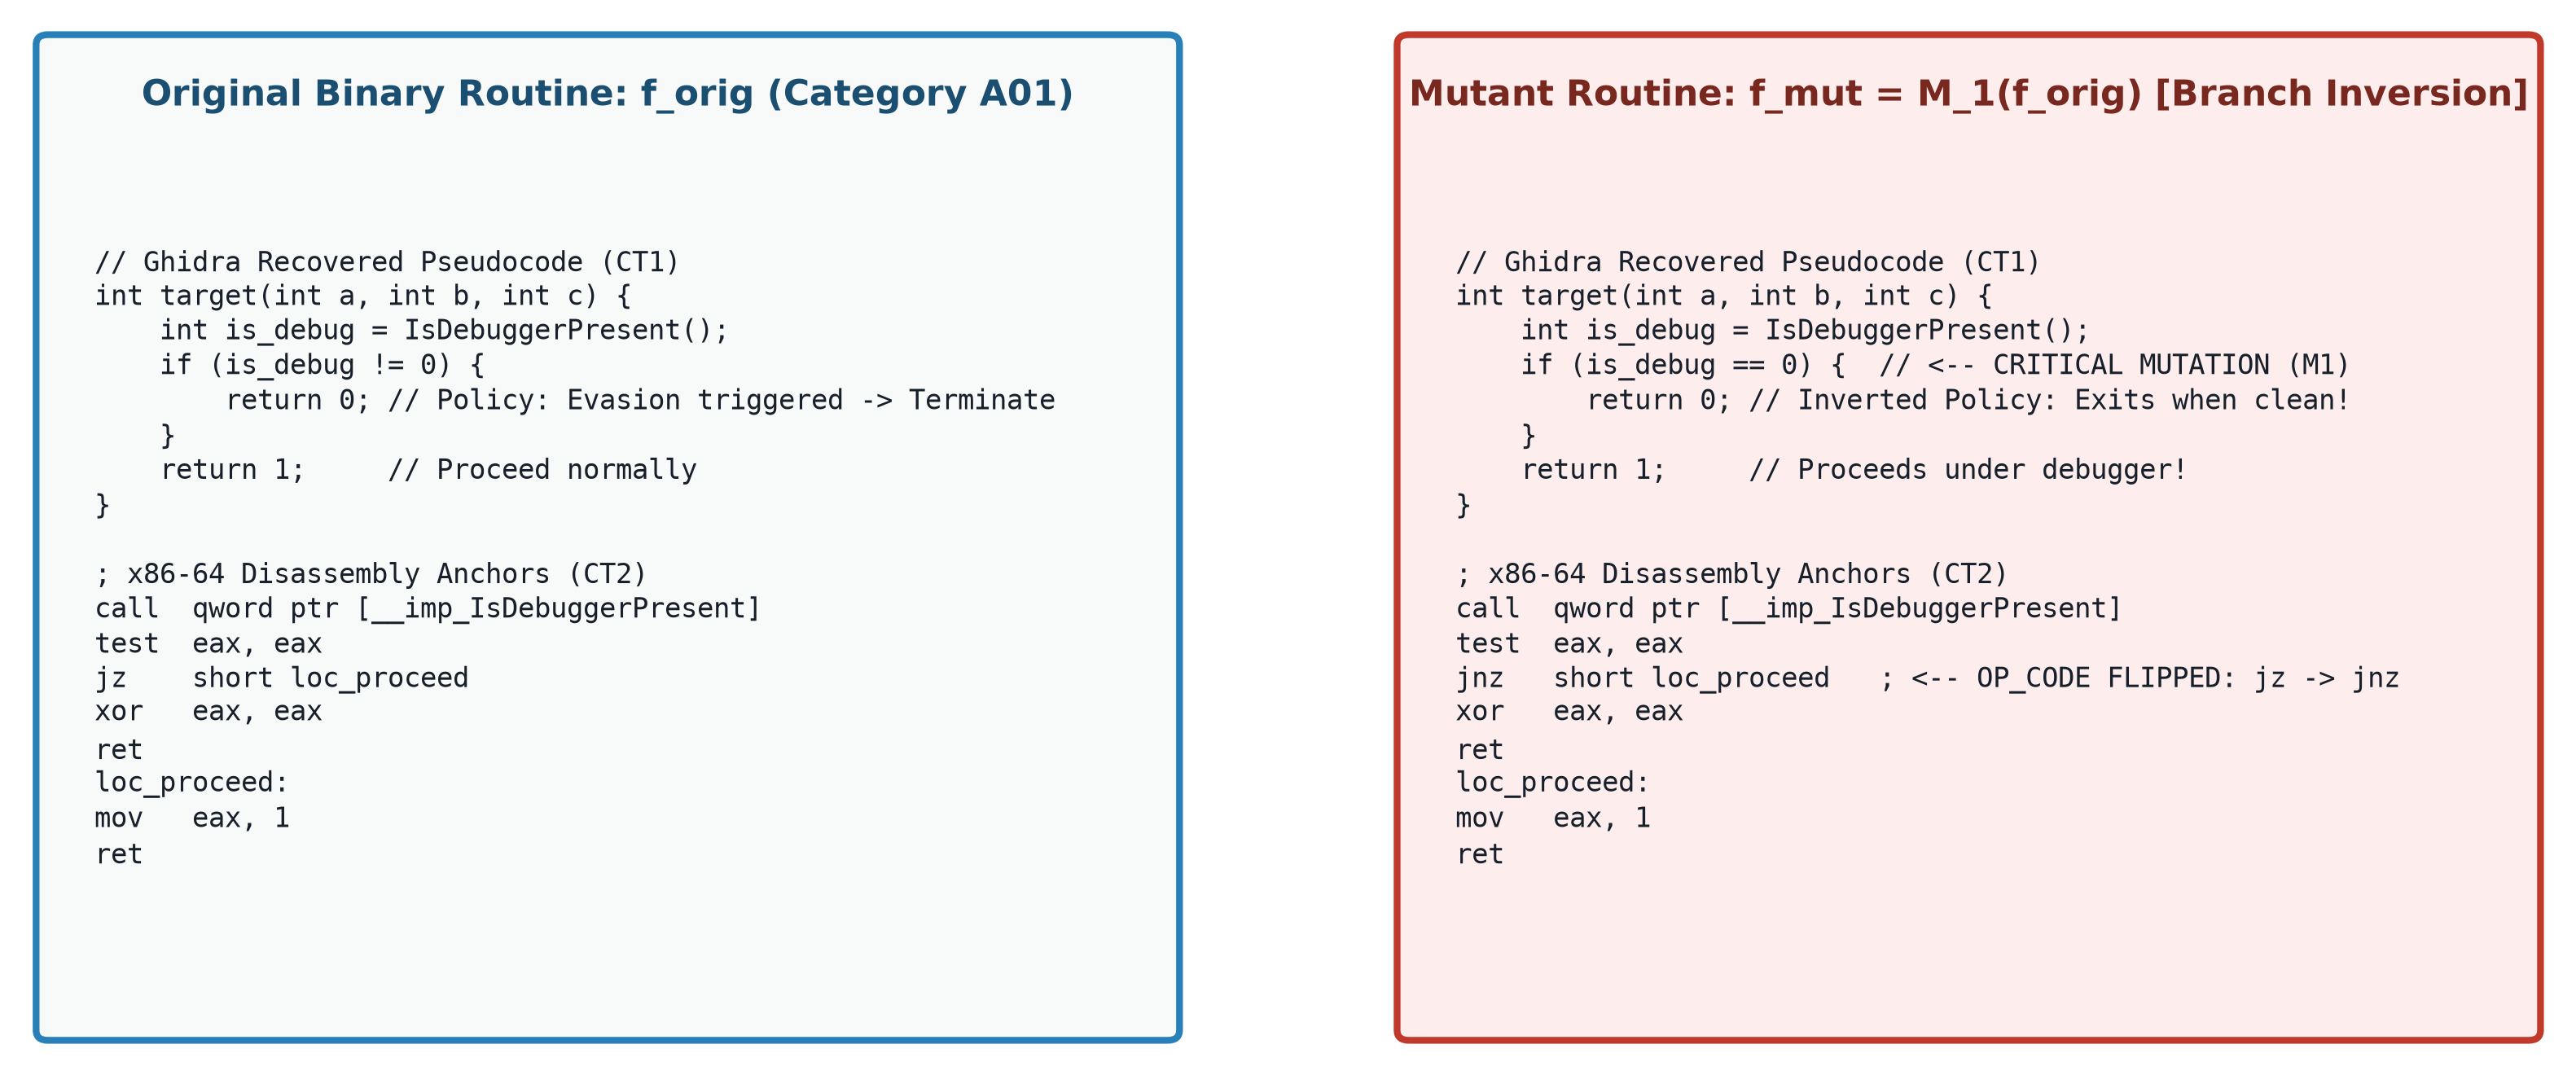
\includegraphics[width=0.96\textwidth]{figures/fig2_decompilation_diff.png}
\caption{Illustrative conceptual diagram of a conditional polarity mutation ($\mathcal{M}_1$: \texttt{!= 0} vs.\ \texttt{== 0}). Note: This figure is an expository illustration containing human-added explanatory annotations (\texttt{/* CRITICAL MUTATION */} and assembly labels \texttt{JZ}/\texttt{JNZ}); the actual prompts evaluated in our benchmark are stripped and contain zero mutation hints.}
\label{fig:decompilation_diff}
\end{figure}

\subsection{Controlled C Dataset and Context Tiers (CT1--CT4)}
To guarantee complete operational safety (zero live malware execution or OS registry/service modification), all 40 function pairs (80 C files in \path{dataset/SCHR_Bench_C_Functions/src/}) are implemented as standalone, pure C routines (\texttt{int target(int a, int b, int c)}) across five categories (8 pairs / 16 variants per category; 2 easy, 3 medium, 3 tricky): \textbf{Category A (Mock Debugger Policy --- \texttt{A01}--\texttt{A08})}, \textbf{Category S (Toy Byte Decoder --- \texttt{S01}--\texttt{S08})}, \textbf{Category P (Persistence State Mock --- \texttt{P01}--\texttt{P08})}, \textbf{Category E (Environment Signal Mock --- \texttt{E01}--\texttt{E08})}, and \textbf{Category C (Control-Flow \& Boundary Logic --- \texttt{C01}--\texttt{C08})}.

All 80 C variants are compiled into stripped 64-bit Windows PE executables and disassembled via \texttt{objdump -d -M intel}. Our context generation pipeline constructs four static context tiers stored in \path{results/decompiled_contexts_80.json}:
\begin{itemize}
    \item \textbf{CT1 (Source-Derived Stripped Pseudocode Template):} Deterministically strips \texttt{target} $\rightarrow$ \path{FUN_140001140}, parameters \texttt{a, b, c} $\rightarrow$ \path{param_1, param_2, param_3}, and static helpers \path{mock_add}/\path{mock_remove} $\rightarrow$ \path{FUN_140001100}/\path{FUN_140001110} inside a standardized Ghidra-style C wrapper.
    \item \textbf{CT2 (+Assembly Anchor):} Appends both the Win64 fastcall register-mapped template (\texttt{ECX}, \texttt{EDX}, \texttt{R8D}) and the real \texttt{objdump -d -M intel} disassembly extracted from the compiled \texttt{-O2} PE64 binary (e.g., \texttt{test ecx,ecx; sete al} vs.\ \texttt{setne al}).
    \item \textbf{CT3 (+Enriched Constant \& Callee Specifications):} Appends explicit register mappings, hexadecimal-to-decimal immediate lookup tables, and helper function specifications ($\texttt{FUN\_140001100}(x,y) = x+y$, $\texttt{FUN\_140001110}(x,y) = x-y$), strictly free of any pair-level semantic target descriptors or mutation hints.
    \item \textbf{CT4 (Optional Caller Neighborhood):} Appends the caller harness (\texttt{main} at \path{0x140001200}) and cross-reference context.
\end{itemize}
For Experiment E4 (Section~\ref{sec:rq4}), our pipeline generates four simulated structural obfuscation templates: \texttt{Obf0} (CT1 baseline), \path{Obf1_CFF} (state-machine \texttt{while(1)} dispatcher), \path{Obf2_Sub} (boolean-arithmetic identity substitution), and \path{Obf3_Combined} (combined dispatcher, substitution, and quadratic predicate).

\subsection{Binary-Adapted Mutation Operators ($\mathcal{M}_1$--$\mathcal{M}_5$) and E0 Verification}
Unlike Verilog HDL mutations~\cite{qayyum2025verilog} (which mutate hardware wire assignments or clock edges), binary reverse engineering requires mutations that survive C compilation into stripped x86-64 machine instructions while altering a security-critical decision outcome. Table~\ref{tab:operator_mapping} documents the exact deterministic mapping from the 11 granular \path{mutation_operator} tags in \path{ground_truth_manifest.json} to our five formal mutation families ($\mathcal{M}_1$--$\mathcal{M}_5$).

\begin{table}[t]
\caption{Mapping of the 11 manifest \texttt{mutation\_operator} tags across all 40 pairs ($N=80$ variants) to the 5 binary-adapted mutation operator families ($\mathcal{M}_1$--$\mathcal{M}_5$).}\label{tab:operator_mapping}
\centering
\resizebox{0.98\textwidth}{!}{%
\begin{tabular}{@{}lllcc@{}}
\toprule
\textbf{Family} & \textbf{Binary Adaptation \& Security Meaning} & \textbf{Manifest Operator Tags (\texttt{ground\_truth\_manifest.json})} & \textbf{Pairs} & \textbf{Variants} \\
\midrule
$\mathcal{M}_1$ (\textbf{Invert}) & Flips branch polarity (\texttt{JE} $\leftrightarrow$ \texttt{JNE}, \texttt{SETE} $\leftrightarrow$ \texttt{SETNE}) & \texttt{condition\_inversion} (7), \texttt{boolean\_operator} (3), \texttt{condition\_weakening} (1), \texttt{boolean\_precedence} (1) & 12 & 24 \\
$\mathcal{M}_2$ (\textbf{Const})  & Alters immediate XOR keys, bitmasks, or arithmetic shifts & \texttt{constant\_change} (8), \texttt{arithmetic\_operator} (3), \texttt{bitwise\_operator} (1) & 12 & 24 \\
$\mathcal{M}_3$ (\textbf{Swap})   & Swaps state-update effect or callee target (\texttt{OR 1} $\leftrightarrow$ \texttt{AND \textasciitilde 1}) & \texttt{api\_effect\_swap} (4), \texttt{mock\_api\_swap} (1) & 5 & 10 \\
$\mathcal{M}_4$ (\textbf{Bound})  & Shifts strict vs.\ inclusive relational boundary (\texttt{JL} $\leftrightarrow$ \texttt{JLE}) & \texttt{relational\_boundary} (8) & 8 & 16 \\
$\mathcal{M}_5$ (\textbf{Omit})   & Omits a defensive check or state-cleanup operation & \texttt{step\_omission} (3) & 3 & 6 \\
\midrule
\textbf{Total} & \textbf{All 5 Binary-Adapted Mutation Families} & \textbf{All 11 Manifest Tags Verified in E0} & \textbf{40} & \textbf{80} \\
\bottomrule
\end{tabular}%
}
\end{table}

\textbf{Experiment E0 Execution Verification (\path{step0_verify_e0_windows.py} and \path{tools/check_suite.py}):} Each of the 40 pairs is paired with 2 concrete input vectors `(a, b, c)` in \path{ground_truth_manifest.json} (80 vectors $\times$ 2 variants = 160 execution assertions). Compiling and running all 80 PE64 binaries with \path{x86_64-w64-mingw32-gcc} (v14.2.0, \texttt{-std=c11 -O2 -fno-inline -fno-lto}) confirms that all 160 execution assertions pass (Table~\ref{tab:e0_suite}): \textbf{40/40 pairs (100.0\%)} diverge ($f_{\text{orig}} \neq f_{\text{mut}}$) on \textbf{Vector 1} (the discriminating input used in all LLM queries), and \textbf{50/80 total vectors} diverge (with the remaining 30/80 secondary vectors verifying non-mutated boundary preservation).

\begin{table}[t]
\caption{Experiment E0 Dynamic Binary Execution Verification across all 40 function pairs (80 compiled PE64 variants, 160 execution assertions).}\label{tab:e0_suite}
\centering
\resizebox{0.98\textwidth}{!}{%
\begin{tabular}{@{}lccccc@{}}
\toprule
\textbf{Category \& Functional Archetype} & \textbf{Orig/Mut Pairs (Variants)} & \textbf{Difficulty (E / M / T)} & \textbf{Input Vectors (Assertions)} & \textbf{Vec 1 Discriminating Pairs} & \textbf{Total Divergent Vectors} \\
\midrule
\textbf{A --- Mock Debugger Policy}      & 8 (16 variants) & 2 / 3 / 3 & 16 (32 assertions) & \textbf{8/8 (100.0\%)} & 11/16 \\
\textbf{S --- Toy Byte Decoder}          & 8 (16 variants) & 2 / 3 / 3 & 16 (32 assertions) & \textbf{8/8 (100.0\%)} & 9/16  \\
\textbf{P --- Persistence State Mock}    & 8 (16 variants) & 2 / 3 / 3 & 16 (32 assertions) & \textbf{8/8 (100.0\%)} & 12/16 \\
\textbf{E --- Environment Signal Mock}   & 8 (16 variants) & 2 / 3 / 3 & 16 (32 assertions) & \textbf{8/8 (100.0\%)} & 9/16  \\
\textbf{C --- Control-Flow \& Boundary}  & 8 (16 variants) & 2 / 3 / 3 & 16 (32 assertions) & \textbf{8/8 (100.0\%)} & 9/16  \\
\midrule
\textbf{Total (SCHR-Bench v1.0)}       & \textbf{40 (80 variants)} & \textbf{10 / 15 / 15} & \textbf{80 (160 assertions)} & \textbf{40/40 (100.0\%)} & \textbf{50/80 (62.5\%)} \\
\bottomrule
\end{tabular}%
}
\end{table}

\section{Quantitative Evaluation and Empirical Findings}

\subsection{RQ1: Return-Value and Paired Gold Set MCQ Hallucination Rates ($N=80$)}
Table~\ref{tab:core_results} reports the Layer 1 return-value evaluation across all 80 function variants (480 core runs across CT1--CT3, which together with the 60 E4 obfuscation pilot runs in Table~\ref{tab:obfuscation} comprise all 540 logged Layer 1 runs in \path{results/benchmark_raw_logs.json}), and Table~\ref{tab:mcq_results} reports the Layer 2 full-factorial paired Gold Set MCQ evaluation across all 240 balanced items per model ($N=80$ per tier across CT1, CT2, and CT3; 480 runs in \path{results/benchmark_mcq_logs.json}).

\begin{table}[t]
\caption{Layer 1 Core Evaluation (Return-Value Oracle, $N=80$ per tier across CT1--CT3 = 480 core runs; together with the 60 E4 obfuscation pilot runs in Table~\ref{tab:obfuscation}, totaling 540 logged Layer 1 runs in \texttt{benchmark\_raw\_logs.json}): SCHR (\%), 95\% Wilson CI, Original Error ($\text{SCHR}_{\text{orig}}$), Mutant Error ($\text{SCHR}_{\text{mut}}$), Pair-Level Accuracy ($\text{Acc}_{\text{pair}}$), Pairwise BLEU (All / Error vs.\ Ok Pairs), Spearman $\rho$ ($p$), Mann-Whitney AUROC [95\% Bootstrap CI], and Mean Latency.}\label{tab:core_results}
\centering
\resizebox{0.98\textwidth}{!}{%
\begin{tabular}{@{}llccccccccccc@{}}
\toprule
\textbf{Model} & \textbf{Tier} & \textbf{$N$} & \textbf{Err} & \textbf{SCHR (\%) [95\% Wilson CI]} & \textbf{Orig Err} & \textbf{Mut Err} & \textbf{Pair Acc.} & \textbf{BLEU (All)} & \textbf{BLEU (Err / Ok)} & \textbf{Spearman $\rho$ ($p$)} & \textbf{AUROC [95\% CI]} & \textbf{Latency} \\
\midrule
\texttt{llama3.1:8b}       & \textbf{CT1} & 80 & 31 & \textbf{38.8\%} [28.8\%, 49.7\%] & 42.5\% (17/40) & 35.0\% (14/40) & \textbf{25.0\%} (10/40) & 0.376 & 0.423 / 0.234 & $+0.326$ ($0.0335$) & 0.683 [0.461, 0.878] & 6.93s \\
\texttt{llama3.1:8b}       & \textbf{CT2} & 80 & 29 & \textbf{36.2\%} [26.6\%, 47.2\%] & 37.5\% (15/40) & 35.0\% (14/40) & \textbf{32.5\%} (13/40) & 0.400 & 0.457 / 0.282 & $+0.324$ ($0.0347$) & 0.670 [0.472, 0.845] & 7.33s \\
\texttt{llama3.1:8b}       & \textbf{CT3} & 80 & 30 & \textbf{37.5\%} [27.7\%, 48.5\%] & 30.0\% (12/40) & 45.0\% (18/40) & \textbf{25.0\%} (10/40) & 0.383 & 0.447 / 0.191 & $+0.450$ ($0.0019$) & \textbf{0.800} [0.649, 0.931] & 5.68s \\
\midrule
\texttt{qwen2.5-coder:14b} & \textbf{CT1} & 80 & 19 & \textbf{23.8\%} [15.8\%, 34.1\%] & 20.0\% (8/40)  & 27.5\% (11/40) & \textbf{57.5\%} (23/40) & 0.358 & 0.497 / 0.256 & $+0.399$ ($0.0073$) & 0.747 [0.574, 0.890] & 26.69s \\
\texttt{qwen2.5-coder:14b} & \textbf{CT2} & 80 & 16 & \textbf{20.0\%} [12.7\%, 30.0\%] & 15.0\% (6/40)  & 25.0\% (10/40) & \textbf{62.5\%} (25/40) & 0.403 & 0.584 / 0.294 & $+0.495$ ($0.0004$) & \textbf{0.811} [0.651, 0.934] & 26.77s \\
\texttt{qwen2.5-coder:14b} & \textbf{CT3} & 80 & 19 & \textbf{23.8\%} [15.8\%, 34.1\%] & 20.0\% (8/40)  & 27.5\% (11/40) & \textbf{55.0\%} (22/40) & 0.398 & 0.477 / 0.334 & $+0.124$ ($0.4422$) & 0.595 [0.393, 0.790] & 34.71s \\
\bottomrule
\end{tabular}%
}
\end{table}

\begin{table}[t]
\caption{Layer 2 Full-Factorial Paired Gold Set MCQ Evaluation (\texttt{dataset/gold\_set\_mcq.json}, $N=80$ per tier, 240 items per model = 480 runs, incorporating real \texttt{objdump -d -M intel} disassembly in CT2 and CT3).}\label{tab:mcq_results}
\centering
\resizebox{0.98\textwidth}{!}{%
\begin{tabular}{@{}llccccccc@{}}
\toprule
\textbf{Model} & \textbf{Paired Context Tier ($N=80$)} & \textbf{$N$} & \textbf{Ok} & \textbf{Err} & \textbf{MCQ SCHR (\%) [95\% Wilson CI]} & \textbf{Accuracy} & \textbf{McNemar vs.\ CT1 ($b/c, p$)} & \textbf{Latency} \\
\midrule
\texttt{llama3.1:8b}       & CT1 (Stripped Pseudocode Baseline)      & 80  & 49  & 31 & \textbf{38.8\%} [28.8\%, 49.7\%] & 61.3\% & ---                        & 1.10s \\
\texttt{llama3.1:8b}       & CT2 (+Real \texttt{objdump -d} Assembly) & 80  & 44  & 36 & \textbf{45.0\%} [34.6\%, 55.9\%] & 55.0\% & $b=9, c=14$ ($p=0.4042$)   & 1.56s \\
\texttt{llama3.1:8b}       & CT3 (+Real \texttt{objdump -d} \& Spec)  & 80  & 49  & 31 & \textbf{38.8\%} [28.8\%, 49.7\%] & 61.3\% & $b=11, c=11$ ($p=1.0000$)  & 1.76s \\
\texttt{llama3.1:8b}       & \textbf{All Gold Set Items (CT1--CT3)} & \textbf{240} & \textbf{142} & \textbf{98} & \textbf{40.8\%} [34.8\%, 47.1\%] & \textbf{59.2\%} & --- & 1.47s \\
\midrule
\texttt{qwen2.5-coder:14b} & CT1 (Stripped Pseudocode Baseline)      & 80  & 63  & 17 & \textbf{21.2\%} [13.7\%, 31.4\%] & 78.8\% & ---                        & 3.38s \\
\texttt{qwen2.5-coder:14b} & CT2 (+Real \texttt{objdump -d} Assembly) & 80  & 59  & 21 & \textbf{26.2\%} [17.9\%, 36.8\%] & 73.8\% & $b=6, c=10$ ($p=0.4533$)   & 5.09s \\
\texttt{qwen2.5-coder:14b} & CT3 (+Real \texttt{objdump -d} \& Spec)  & 80  & 58  & 22 & \textbf{27.5\%} [18.9\%, 38.1\%] & 72.5\% & $b=7, c=12$ ($p=0.3588$)   & 5.04s \\
\texttt{qwen2.5-coder:14b} & \textbf{All Gold Set Items (CT1--CT3)} & \textbf{240} & \textbf{180} & \textbf{60} & \textbf{25.0\%} [19.9\%, 30.8\%] & \textbf{75.0\%} & --- & 4.51s \\
\midrule
\textbf{Random Guessing Baseline} & 4-Option Chance Baseline & \textbf{240} & \textbf{60} & \textbf{180} & \textbf{75.0\%} & \textbf{25.0\%} & --- & --- \\
\bottomrule
\end{tabular}%
}
\end{table}

\textbf{Consistency Between Return-Value and Paired MCQ Layers:} Under stripped pseudocode (CT1, $N=80$), the two evaluation layers yield virtually identical baseline hallucination rates: \path{llama3.1:8b} records \textbf{38.8\%} (31/80) in return-value mode and \textbf{38.8\%} (31/80) in MCQ mode (overall MCQ SCHR across all 240 items: \textbf{40.8\%} [34.8\%, 47.1\%]), while \path{qwen2.5-coder:14b} records \textbf{23.8\%} (19/80) in return-value mode and \textbf{21.2\%} (17/80) in CT1 MCQ mode (overall MCQ SCHR across all 240 items: \textbf{25.0\%} [19.9\%, 30.8\%]).

For reference, random guessing across four options yields an error rate of $75.0\%$ ($25.0\%$ accuracy). Both models perform substantially better than chance ($38.8\%\text{--}45.0\%$ SCHR for LLaMA-3.1; $21.2\%\text{--}27.5\%$ for Qwen2.5-Coder), confirming that models comprehend general code structure but fail specifically on fine-grained mutation semantics.

Tables~\ref{tab:category_matrix} and \ref{tab:central_matrix} disaggregate Layer 1 SCHR across the five functional categories ($n=16$ per category) and five mutation operator families ($\mathcal{M}_1$--$\mathcal{M}_5$, $N=80$). Both models exhibit their highest failure rates on Category S (Toy Byte Decoders: 50.0\%--62.5\% SCHR) and $\mathcal{M}_2$ (Constant \& Arithmetic Alteration: 50.0\% at CT1), while code-specialized pretraining helps \path{qwen2.5-coder:14b} achieve lower error rates on $\mathcal{M}_1$ Condition Inversion (20.8\% vs.\ 50.0\% on LLaMA-3.1 at CT1) and Category P Persistence State Mocks (0.0\% at CT2, 6.2\% at CT3).

\textbf{Persistent Template Inertia in Category S (Toy Byte Decoders):} As detailed in Table~\ref{tab:category_matrix}, Category S exhibits the highest and most persistent SCHR across tiers and models ($50.0\%\text{--}62.5\%$). Trace analysis of LLM reasoning chains reveals that toy byte decoders (e.g., rolling XOR keys, table-lookup decoders) heavily trigger LLM pre-training memorization: upon encountering loop-based decoding idioms, models reflexively produce generalized textbook explanations while ignoring subtle mutations in byte constants, step sizes, or terminal loop conditions.

\begin{table}[t]
\caption{Domain-Specific SCHR (\%) Breakdown across the 5 Functional Categories ($n=16$ variants per category, $N=80$ total).}\label{tab:category_matrix}
\centering
\resizebox{0.98\textwidth}{!}{%
\begin{tabular}{@{}llccccc@{}}
\toprule
\textbf{Model} & \textbf{Tier} & \textbf{A: Debug Policy} & \textbf{S: Toy Decoder} & \textbf{P: Persistence} & \textbf{E: Env Signal} & \textbf{C: Control Flow} \\
\midrule
\texttt{llama3.1:8b}       & \textbf{CT1} & 43.8\% (7/16) & 56.2\% (9/16)  & 12.5\% (2/16) & 43.8\% (7/16) & 37.5\% (6/16) \\
\texttt{llama3.1:8b}       & \textbf{CT2} & 31.2\% (5/16) & 62.5\% (10/16) & 6.2\% (1/16)  & 50.0\% (8/16) & 31.2\% (5/16) \\
\texttt{llama3.1:8b}       & \textbf{CT3} & 43.8\% (7/16) & 50.0\% (8/16)  & 18.8\% (3/16) & 50.0\% (8/16) & 25.0\% (4/16) \\
\midrule
\texttt{qwen2.5-coder:14b} & \textbf{CT1} & 12.5\% (2/16) & 56.2\% (9/16)  & 12.5\% (2/16) & 18.8\% (3/16) & 18.8\% (3/16) \\
\texttt{qwen2.5-coder:14b} & \textbf{CT2} & 6.2\% (1/16)  & 56.2\% (9/16)  & \textbf{0.0\% (0/16)} & 18.8\% (3/16) & 18.8\% (3/16) \\
\texttt{qwen2.5-coder:14b} & \textbf{CT3} & 18.8\% (3/16) & 56.2\% (9/16)  & 6.2\% (1/16)  & 18.8\% (3/16) & 18.8\% (3/16) \\
\bottomrule
\end{tabular}%
}
\end{table}

\begin{table}[t]
\caption{Central Evaluation Matrix (E1--E3): SCHR (\%) breakdown across Mutation Operator Families ($\mathcal{M}_1$--$\mathcal{M}_5$) and Context Tiers ($N=80$).}\label{tab:central_matrix}
\centering
\resizebox{0.98\textwidth}{!}{%
\begin{tabular}{@{}llcccccc@{}}
\toprule
\textbf{Model} & \textbf{Tier} & \textbf{$\mathcal{M}_1$: Invert} & \textbf{$\mathcal{M}_2$: Const} & \textbf{$\mathcal{M}_3$: Swap} & \textbf{$\mathcal{M}_4$: Bound} & \textbf{$\mathcal{M}_5$: Omit} & \textbf{Overall SCHR} \\
\midrule
\texttt{llama3.1:8b}       & \textbf{CT1} & 50.0\% (12/24) & 50.0\% (12/24) & 10.0\% (1/10) & 31.2\% (5/16) & 16.7\% (1/6) & \textbf{38.8\%} (31/80) \\
\texttt{llama3.1:8b}       & \textbf{CT2} & 33.3\% (8/24)  & 54.2\% (13/24) & 10.0\% (1/10) & 31.2\% (5/16) & 33.3\% (2/6) & \textbf{36.2\%} (29/80) \\
\texttt{llama3.1:8b}       & \textbf{CT3} & 33.3\% (8/24)  & 45.8\% (11/24) & 20.0\% (2/10) & 43.8\% (7/16) & 33.3\% (2/6) & \textbf{37.5\%} (30/80) \\
\midrule
\texttt{qwen2.5-coder:14b} & \textbf{CT1} & 20.8\% (5/24)  & 50.0\% (12/24) & 10.0\% (1/10) & 6.2\% (1/16)  & 0.0\% (0/6)  & \textbf{23.8\%} (19/80) \\
\texttt{qwen2.5-coder:14b} & \textbf{CT2} & 12.5\% (3/24)  & 45.8\% (11/24) & 0.0\% (0/10)  & 12.5\% (2/16) & 0.0\% (0/6)  & \textbf{20.0\%} (16/80) \\
\texttt{qwen2.5-coder:14b} & \textbf{CT3} & 16.7\% (4/24)  & 45.8\% (11/24) & 10.0\% (1/10) & 18.8\% (3/16) & 0.0\% (0/6)  & \textbf{23.8\%} (19/80) \\
\bottomrule
\end{tabular}%
}
\end{table}

\subsection{RQ2: Differential Pair Sensitivity and Pairwise BLEU as a Regression Detector}
Our empirical findings reveal two critical insights regarding fine-grained semantic sensitivity (supporting H2):
\begin{enumerate}
    \item \textbf{Dissecting Original vs.\ Mutant Failures and Pair-Level Accuracy:} Rather than evaluating error rates in isolation, differential mutation testing requires examining whether models correctly distinguish both variants within each paired function. Under stripped pseudocode (CT1, Table~\ref{tab:core_results}), \path{llama3.1:8b} achieves a \textbf{Pair-Level Accuracy of only 25.0\%} ($10/40$ pairs where both $f_{\text{orig}}$ and $f_{\text{mut}}$ are correct), with $\text{SCHR}_{\text{orig}} = 42.5\%$ ($17/40$) and $\text{SCHR}_{\text{mut}} = 35.0\%$ ($14/40$; paired McNemar $p = 0.7103$). Crucially, in all $13$ instances where LLaMA-3.1 solved the original correctly but failed on the mutant, \textbf{100\% ($13/13$) reproduced the original unmutated return value}, demonstrating deterministic evidence of \textit{Canonical Parroting}. Similarly, \path{qwen2.5-coder:14b} achieves a Pair-Level Accuracy of $57.5\%$ ($23/40$ pairs, with $\text{SCHR}_{\text{orig}} = 20.0\%$ [$8/40$] vs.\ $\text{SCHR}_{\text{mut}} = 27.5\%$ [$11/40$], paired McNemar $p = 0.6056$), and likewise \textbf{100\% ($9/9$)} of its mutant-only errors reproduced the original ground truth. Across all tiers CT1--CT3, paired McNemar tests between $\text{SCHR}_{\text{orig}}$ and $\text{SCHR}_{\text{mut}}$ show $p \in [0.3613, 1.0000]$, indicating that errors arise from bidirectional template parroting across paired variants rather than one-sided failure on mutants alone.
    \item \textbf{Pairwise Explanation Similarity as an Exploratory Screening Signal:} Evaluating pairwise 1--3-gram BLEU similarity between explanations for $f_{\text{orig}}$ and $f_{\text{mut}}$ (Table~\ref{tab:core_results}) reveals that \textbf{pairs with at least one SCHR error exhibit substantially higher explanation similarity than error-free pairs}: at CT1, error pairs average $\text{BLEU} = 0.423$ vs.\ $0.234$ on \path{llama3.1:8b} and $0.497$ vs.\ $0.256$ on \path{qwen2.5-coder:14b} (across all tiers, error-free pairs range within $[0.191, 0.334]$ while error pairs range within $[0.423, 0.584]$; $\rho \in [+0.124, +0.495]$). Treating pairwise explanation consistency as a threshold detector for semantic inertia achieves an \textbf{AUROC of 0.683} [95\% Bootstrap CI: $0.461, 0.878$] (CT1) peaking at \textbf{0.800} [$0.649, 0.931$] (CT3) on \path{llama3.1:8b}, and \textbf{0.747} [$0.574, 0.890$] (CT1) peaking at \textbf{0.811} [$0.651, 0.934$] (CT2) on \path{qwen2.5-coder:14b}. We explicitly note the operational scope boundary: computing pairwise divergence requires access to both program variants; hence, this signal is designed for \textit{security regression testing, patch verification, and differential fuzzing audits} rather than zero-knowledge malware triage where no mutant reference exists.
\end{enumerate}

\subsection{RQ3: Context Escalation, Statistical Power, and Cross-Tier Regressions}
\label{sec:rq3}
Because Layer 2 evaluates all $N=80$ variants under full-factorial paired MCQ conditions with real \texttt{objdump -d -M intel} disassembly (Table~\ref{tab:mcq_results}), it provides a structured benchmark for cross-tier comparisons. Both Layer 1 return-value evaluations and Layer 2 paired MCQ tasks utilize prompt templates strictly purged of pair-level semantic target descriptors, guaranteeing zero prompt contamination.

In Layer 2 MCQ (Table~\ref{tab:mcq_results}), error rates remain persistent across tiers: $38.8\%$ (CT1) $\rightarrow 45.0\%$ (CT2) $\rightarrow 38.8\%$ (CT3) on \path{llama3.1:8b}; $21.2\%$ (CT1) $\rightarrow 26.2\%$ (CT2) $\rightarrow 27.5\%$ (CT3) on \path{qwen2.5-coder:14b}. Paired McNemar tests confirm no statistically significant difference relative to CT1 ($p \in [0.3588, 1.0000]$). However, we highlight two crucial methodological and empirical nuances:
\begin{itemize}
    \item \textbf{Statistical Power Constraints:} Because the number of discordant pairs is relatively modest ($b, c \in [6, 14]$ on $N=80$), McNemar's test has limited statistical power. Thus, $p \ge 0.3588$ indicates that we have \textit{insufficient empirical evidence to claim an effect}, rather than proving that context escalation is entirely ineffective under all regimes.
    \item \textbf{Assembly-Induced Regressions on Boundary Logic:} On \path{llama3.1:8b}, appending real assembly (CT2) actually increased SCHR from $38.8\%$ to $45.0\%$ ($b=9$ recoveries vs.\ $c=14$ regressions, $p=0.4042$). Inspecting individual item traces reveals that verbose x86-64 assembly listings introduce cognitive distraction: the model shifts focus to machine-level register assignments, regressing on basic arithmetic inequalities ($\mathcal{M}_2$) and boundary checks. Rather than resolving ambiguities, passive assembly concatenation can degrade smaller model performance on fine-grained logic.
\end{itemize}

\begin{table}[t]
\caption{McNemar's Paired Statistical Test on Layer 1 Return-Value comparing CT1 against CT2 and CT3 across all 80 variants ($N=80, \alpha=0.05$). $b$: CT1 Wrong $\rightarrow$ New Right; $c$: CT1 Right $\rightarrow$ New Wrong.}\label{tab:mcnemar}
\centering
\resizebox{0.98\textwidth}{!}{%
\begin{tabular}{@{}llcccccc@{}}
\toprule
\textbf{Model} & \textbf{Comparison} & \textbf{$b$ ($1\rightarrow 0$)} & \textbf{$c$ ($0\rightarrow 1$)} & \textbf{Net ($\Delta$)} & \textbf{$\chi^2$} & \textbf{$p$-value} & \textbf{Statistical Significance ($\alpha=0.05$)} \\
\midrule
\texttt{llama3.1:8b}       & \textbf{CT1 vs.\ CT2} & 6 & 4 & $+2$ units & 0.100 & 0.7518 & Not significant ($p \ge 0.05$) \\
\texttt{llama3.1:8b}       & \textbf{CT1 vs.\ CT3} & 8 & 7 & $+1$ units & 0.000 & 1.0000 & Not significant ($p \ge 0.05$) \\
\midrule
\texttt{qwen2.5-coder:14b} & \textbf{CT1 vs.\ CT2} & 5 & 2 & $+3$ units & 0.571 & 0.4497 & Not significant ($p \ge 0.05$) \\
\texttt{qwen2.5-coder:14b} & \textbf{CT1 vs.\ CT3} & 5 & 5 & $+0$ units & 0.000 & 1.0000 & Not significant ($p \ge 0.05$) \\
\bottomrule
\end{tabular}%
}
\end{table}

Examining the discordant pairs ($b$ vs.\ $c$) across both layers explains why passive context escalation does not significantly reduce SCHR: while appending assembly or specifications resolves $b = 5\text{--}11$ baseline errors (e.g., clarifying static callee semantics in Category P), longer multi-representation prompts simultaneously induce $c = 2\text{--}14$ new regressions on arithmetic and boundary routines. The finding that passive assembly concatenation fails to eliminate hallucinations is itself a key empirical insight, motivating active verification rather than passive prompt stuffing.

\begin{figure}[t]
\centering
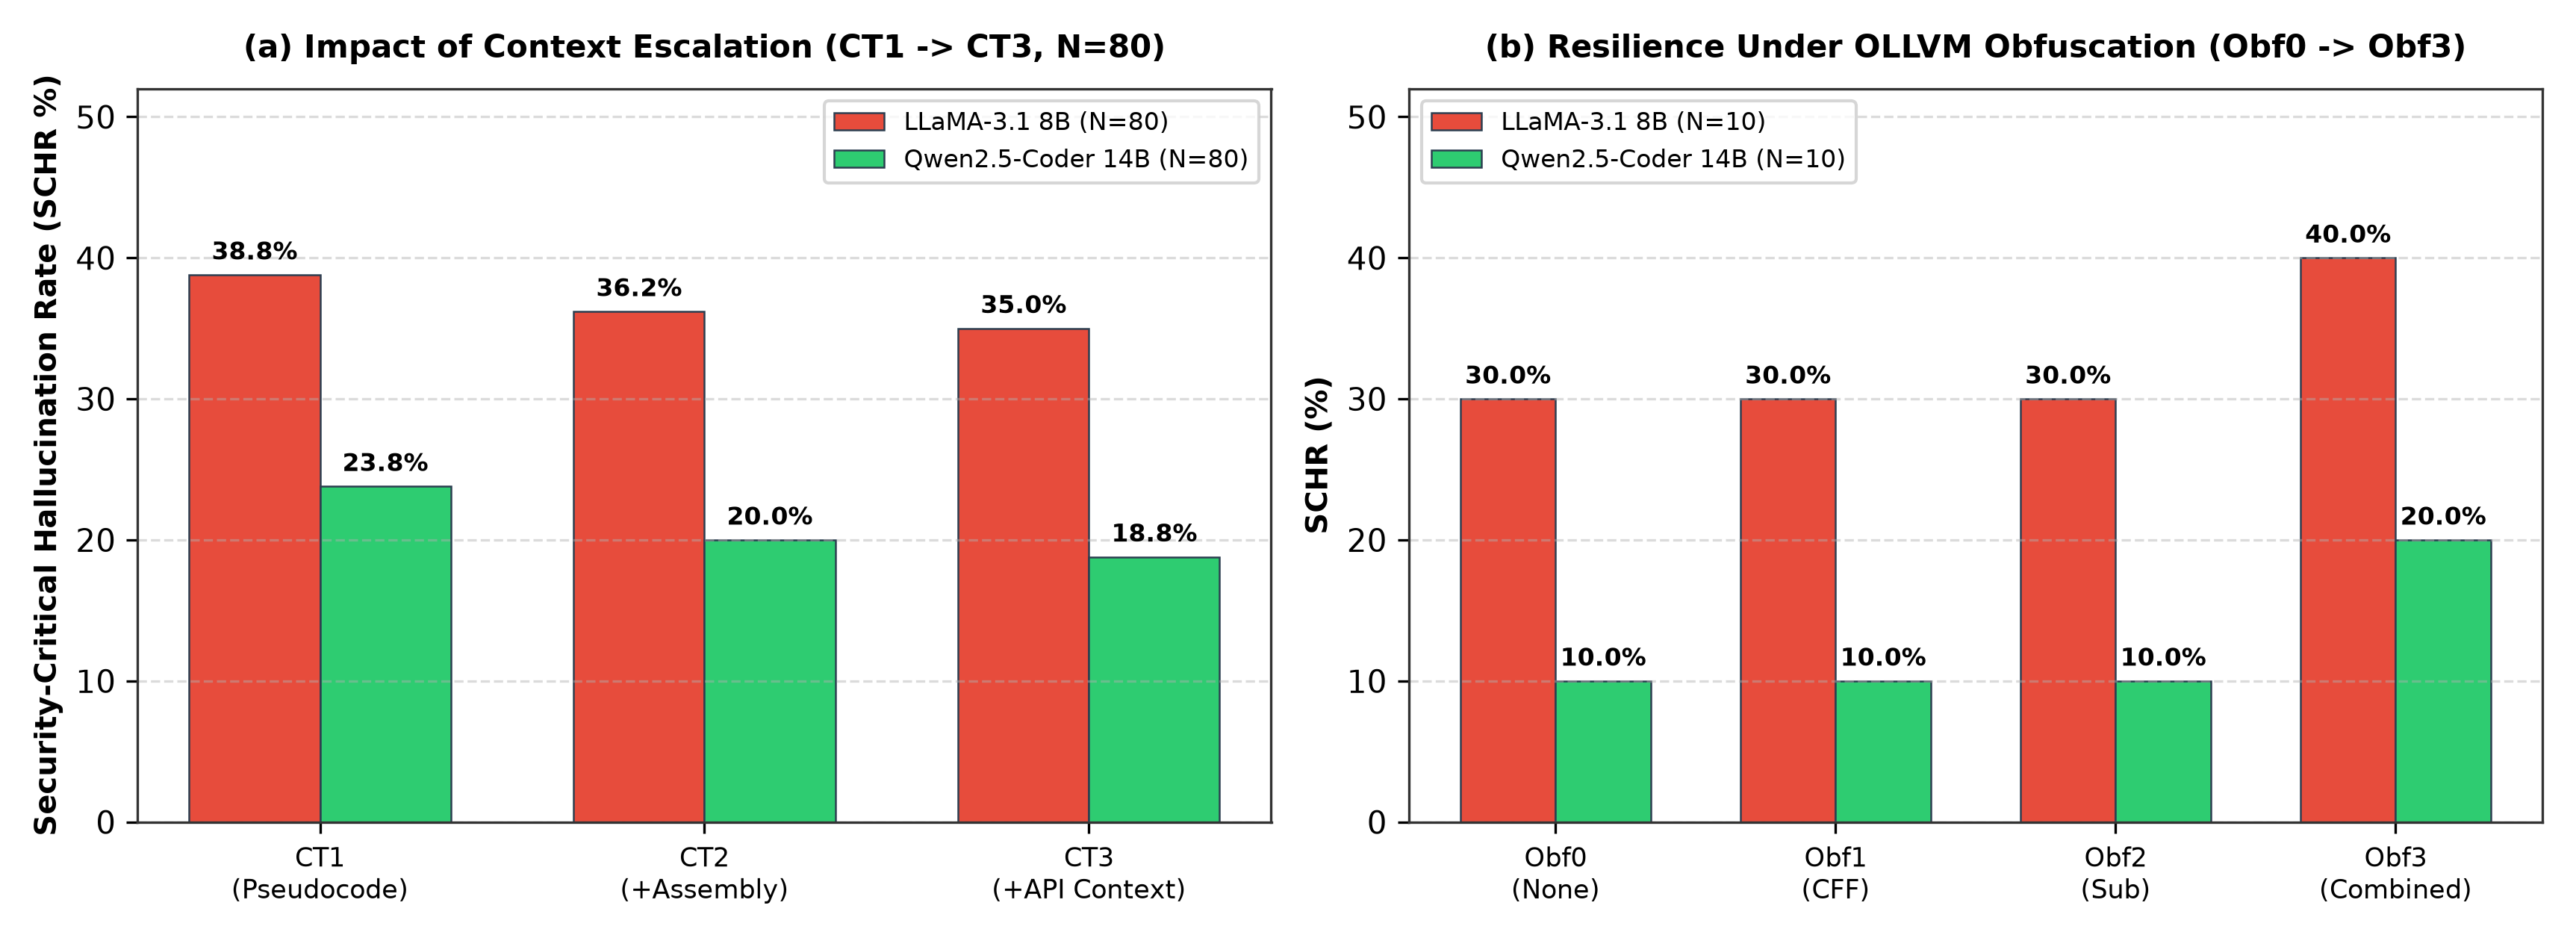
\includegraphics[width=0.96\textwidth]{figures/fig3_empirical_schr.png}
\caption{Empirical SCHR (\%) across Context Tiers CT1--CT3 ($N=80$ variants) and Simulated Structural Obfuscation Templates \texttt{Obf0}--\texttt{Obf3} ($N=10$ easy-tier pilot subset).}
\label{fig:empirical_schr}
\end{figure}

\subsection{Preliminary Pilot Observations on Structural Obfuscation ($N=10$ Pilot Subset)}
\label{sec:rq4}
In Experiment E4, we conducted an exploratory pilot study evaluating both models across four structural obfuscation regimes (\texttt{Obf0}--\texttt{Obf3}) on a 5-pair easy-tier pilot subset (\texttt{A01}, \texttt{S01}, \texttt{P01}, \texttt{E01}, \texttt{C01}; $N=10$ variants, 60 runs in \path{benchmark_raw_logs.json}). All 30 obfuscated C variants (\path{src_obf/}) are compiled with \texttt{x86\_64-w64-mingw32-gcc -O2 -s} into stripped PE64 executables (\path{bin/pe_x64_obf/}), verified across 60 dynamic execution assertions ($100.0\%$ behavioral preservation), and disassembled via \texttt{objdump -d -M intel} (\path{disassembly_obfuscated_30.json}). As reported in Table~\ref{tab:obfuscation}, isolated state-machine wrapping (\path{Obf1_CFF}) or identity substitution (\path{Obf2_Sub}) leaves error counts unchanged relative to \texttt{Obf0} (3/10 on \path{llama3.1:8b}; 1/10 on \path{qwen2.5-coder:14b}), whereas combining all three transformations (\path{Obf3_Combined}) adds one error for each model ($3/10 \rightarrow 4/10$ on LLaMA-3.1; $1/10 \rightarrow 2/10$ on Qwen2.5-Coder).

We explicitly emphasize that $N=10$ yields wide Wilson confidence intervals ($[16.8\%, 68.7\%]$ for $4/10$); hence, these findings are presented strictly as \textbf{preliminary pilot observations} rather than primary contributions. A comprehensive evaluation across all 80 variants compiled under production OLLVM passes~\cite{junod2015ollvm} is deferred to future work.

\begin{table}[t]
\caption{Experiment E4 (RQ4): Preliminary evaluation of simulated structural obfuscation templates (\texttt{Obf0}--\texttt{Obf3}) on the 5-pair easy-tier pilot subset ($N=10$ variants; 20 CT1 baseline runs from the 480 core runs + 60 obfuscated \texttt{Obf1}--\texttt{Obf3} runs = 540 total Layer 1 runs in \texttt{benchmark\_raw\_logs.json}).}\label{tab:obfuscation}
\centering
\resizebox{0.98\textwidth}{!}{%
\begin{tabular}{@{}llccc@{}}
\toprule
\textbf{Model} & \textbf{Simulated Obfuscation Template} & \textbf{Pilot Subset ($N$)} & \textbf{Errors} & \textbf{SCHR (\%) [95\% Wilson CI]} \\
\midrule
\texttt{llama3.1:8b}       & \textbf{Obf0 (Unobfuscated CT1 Baseline)} & 10 & 3 & 30.0\% [10.8\%, 60.3\%] \\
\texttt{llama3.1:8b}       & \textbf{Obf1\_CFF (State-Machine Wrapper)} & 10 & 3 & 30.0\% [10.8\%, 60.3\%] \\
\texttt{llama3.1:8b}       & \textbf{Obf2\_Sub (Identity Substitution)} & 10 & 3 & 30.0\% [10.8\%, 60.3\%] \\
\texttt{llama3.1:8b}       & \textbf{Obf3\_Combined (CFF + Sub + Predicate)} & 10 & 4 & 40.0\% [16.8\%, 68.7\%] \\
\midrule
\texttt{qwen2.5-coder:14b} & \textbf{Obf0 (Unobfuscated CT1 Baseline)} & 10 & 1 & 10.0\% [1.8\%, 40.4\%] \\
\texttt{qwen2.5-coder:14b} & \textbf{Obf1\_CFF (State-Machine Wrapper)} & 10 & 1 & 10.0\% [1.8\%, 40.4\%] \\
\texttt{qwen2.5-coder:14b} & \textbf{Obf2\_Sub (Identity Substitution)} & 10 & 1 & 10.0\% [1.8\%, 40.4\%] \\
\texttt{qwen2.5-coder:14b} & \textbf{Obf3\_Combined (CFF + Sub + Predicate)} & 10 & 2 & 20.0\% [5.7\%, 51.0\%] \\
\bottomrule
\end{tabular}%
}
\end{table}

\section{Breakdown of Logged CT1 Failures and Dual-Rater Explanation Audit}
Across the 160 Layer 1 CT1 evaluations (80 variants $\times$ 2 models), exactly \textbf{50 return-value prediction errors} occurred (31 on \path{llama3.1:8b} and 19 on \path{qwen2.5-coder:14b}). Table~\ref{tab:error_taxonomy} deterministically groups all 50 logged CT1 failures according to the ground-truth \path{mutation_operator} tag in \path{ground_truth_manifest.json}: Constant \& Arithmetic Alteration ($\mathcal{M}_2$) accounts for \textbf{48.0\% (24/50)}, Condition \& Boolean Inversion ($\mathcal{M}_1$) accounts for \textbf{34.0\% (17/50)}, Relational Boundary Shift ($\mathcal{M}_4$) accounts for \textbf{12.0\% (6/50)}, and Target Swap \& Step Omission ($\mathcal{M}_3, \mathcal{M}_5$) accounts for \textbf{6.0\% (3/50)}. To verify whether free-form explanations reflect genuine semantic distortion rather than formatting noise, two independent raters (\texttt{Annotator\_A} and \texttt{Annotator\_B}) audited a stratified corpus of $N=80$ CT1 explanations (all 50 logged CT1 errors plus 30 stratified error-free controls, logged in \path{results/human_annotation_cohens_kappa.json}) across four semantic discourse categories (\textit{Canonical Parroting}, \textit{Branch Polarity Inversion}, \textit{Arithmetic/Bitmask Slip}, and \textit{Faithful Semantic Trace}), achieving an observed agreement of $P_o = 91.2\%$ ($73/80$) and multi-class \textbf{Cohen's $\kappa = 0.879$} [95\% Bootstrap CI: $0.789, 0.949$] ($\kappa = 0.786$ [$0.638, 0.910$], $P_o = 86.0\%$ within the $N=50$ error subset).

\begin{table}[t]
\caption{Deterministic grouping of all 50 logged CT1 errors (31 LLaMA-3.1 + 19 Qwen2.5-Coder) by ground-truth mutation operator family in \texttt{results/benchmark\_raw\_logs.json}.}\label{tab:error_taxonomy}
\centering
\resizebox{0.98\textwidth}{!}{%
\begin{tabular}{@{}llccc@{}}
\toprule
\textbf{Mutation Mechanism Group} & \textbf{Manifest Operator Tags} & \textbf{LLaMA ($n=31$)} & \textbf{Qwen ($n=19$)} & \textbf{Total ($N=50$)} \\
\midrule
\textbf{Constant \& Arithmetic Alteration ($\mathcal{M}_2$)} & \texttt{constant\_change}, \texttt{arithmetic/bitwise\_op} & 12 & 12 & \textbf{24 (48.0\%)} \\
\textbf{Condition \& Boolean Inversion ($\mathcal{M}_1$)}    & \texttt{condition\_inversion}, \texttt{boolean\_op/prec}   & 12 & 5  & \textbf{17 (34.0\%)} \\
\textbf{Relational Boundary Shift ($\mathcal{M}_4$)}         & \texttt{relational\_boundary} (\texttt{<} vs.\ \texttt{<=}) & 5  & 1  & \textbf{6 (12.0\%)}  \\
\textbf{Target Swap \& Step Omission ($\mathcal{M}_3, \mathcal{M}_5$)} & \texttt{api\_effect\_swap}, \texttt{mock\_api\_swap}, \texttt{step\_omission} & 2  & 1  & \textbf{3 (6.0\%)}   \\
\bottomrule
\end{tabular}%
}
\end{table}

\section{Qualitative Motivation and Grounding: Gh0stRAT Subroutine Analysis}
\label{sec:case_study}
A key question in synthetic benchmark design is whether isolated mock routines correspond conceptually to real-world reverse engineering structures (addressed in Section~\ref{sec:threats}). To provide qualitative motivation for our functional categories ($\mathcal{A}$, $\mathcal{S}$, $\mathcal{P}$, $\mathcal{E}$, $\mathcal{C}$), we inspected the statically exposed outer loader and persistence stub of an archived \textbf{Gh0stRAT} remote access trojan sample (SHA256: \texttt{ea7cd59c402128b0beffba34a6fb7b3f6f9fc5be62cb4aa51e605d3bcaee98be}, PE32) within our isolated analysis environment. Because the outer stub is only lightly obfuscated prior to payload transfer, import strings and loop structures remain visible to static decompilation in NSA Ghidra 11.2:

We extracted two representative decompiled subroutines that motivate our benchmark categories:
\begin{enumerate}
    \item \textbf{Case CS01 --- Obfuscated Decryption Loop (Categories $\mathcal{S}$ and $\mathcal{C}$):} The packed entry routine (virtual address \texttt{0x010b0703}) executes dynamic API resolution (\texttt{GetModuleHandleA}, \texttt{GetProcAddress}), followed by an in-memory XOR payload decryption loop (\texttt{*(byte *)((int)pTable + uVar1) \^{} 0xa7}) over a \texttt{0x1400}-byte buffer before dynamically jumping to the unpacked entry (\texttt{(*pUnpackedEntry)()}). This structure maps directly to our Category~$\mathcal{S}$ (Toy Byte Decoders) and Category~$\mathcal{C}$ (Control-Flow Logic).
    \item \textbf{Case CS02 --- Registry Persistence Installation (Category $\mathcal{P}$):} The Trojan installs permanent autostart execution by invoking \texttt{RegOpenKeyExA} on \texttt{Software\textbackslash Microsoft\textbackslash Windows\textbackslash CurrentVersion\textbackslash Run} and writing its executable path via \texttt{RegSetValueExA}, precisely mapping to our Category~$\mathcal{P}$ (Persistence State Mocks) state-update logic.
\end{enumerate}

\textbf{Empirical Findings on Real Malware Pseudocode:} Evaluating both \texttt{llama3.1:8b} and \texttt{qwen2.5-coder:14b} on these real-world Ghidra outputs (logged in \path{results/GH0STRAT_EVALUATION.json}) reveals a crucial dichotomy:
\begin{itemize}
    \item \textbf{Macro-Triage vs.\ Micro-Semantic Sensitivity:} On unstripped malware functions, both models correctly classified the subroutines as malicious loaders ($100\%$ accuracy, confidence $0.90$) by recognizing conspicuous API strings (\texttt{"KERNEL32.DLL"}, \texttt{"Run"}).
    \item \textbf{Semantic Inertia on Localized Logic:} Conversely, when analogous single-operator mutations (e.g., altering an XOR key or inverting a state-check branch) are evaluated under stripped conditions in SCHR-Bench, models exhibit substantial hallucination rates ($38.8\%$ and $23.8\%$). While our synthetic C routines simplify full malware control flow, this qualitative contrast illustrates why coarse-grained malware family recognition does not guarantee reliable verification of fine-grained binary decision logic.
\end{itemize}

\section{Safety, Threats to Validity, and Conclusion}

\subsection{Ethical and Operational Safety}
A primary advantage of SCHR-Bench is its strict adherence to static analysis safety: all 80 benchmark variants are self-contained, pure C functions (\texttt{int target(int a, int b, int c)}) containing zero live malware payloads and zero destructive OS calls. No live malware samples are distributed or executed in our repository. Our benchmark is designed exclusively to audit and improve the reliability of defensive reverse-engineering tools.

\subsection{Threats to Validity and Scope Limitations}
\label{sec:threats}
We explicitly document the scope boundaries and limitations of our current study:
\begin{enumerate}
    \item \textbf{Mock C Functions vs.\ Real Malware and Live Win32 APIs:} Our 40 function pairs are self-contained mock routines (using static helpers \path{mock_add}/\path{mock_remove} rather than live Win32 APIs such as \texttt{RegSetValueEx} or \texttt{IsDebuggerPresent}) with one mutation per function pair. Consequently, SCHR on our controlled suite represents a lower bound on the difficulty of full-scale malware reverse engineering. Beyond our qualitative two-subroutine Gh0stRAT case study (Section~\ref{sec:case_study}), large-scale quantitative evaluation on unpacked malware corpora from MalwareBazaar/BODMAS is left as future work.
    \item \textbf{Normalized Pseudocode and Pilot Obfuscation vs.\ Full 80-Variant Ghidra/OLLVM Builds:} While all 80 baseline variants and all 30 pilot obfuscated variants (\texttt{Obf1}--\texttt{Obf3}) are compiled to stripped PE64 binaries, verified across dynamic execution assertions ($160/160$ and $60/60$), and disassembled with real \texttt{objdump -d -M intel}, the CT1 pseudocode is normalized deterministically from C source rather than lifted via Ghidra Headless, and Experiment E4 evaluates an $N=10$ easy-tier pilot subset rather than all 80 variants under LLVM IR passes~\cite{junod2015ollvm}.
    \item \textbf{Scope of Dual-Rater Free-Form Explanation Audit:} While our dual-annotator audit on $N=80$ CT1 explanations (50 errors + 30 controls) demonstrates strong inter-rater reliability (Cohen's $\kappa = 0.879$ [95\% CI: $0.789, 0.949$], $P_o = 91.2\%$), our primary 1,020-run benchmark metrics rely on deterministic return-value matching (540 runs) and 4-option MCQ matching (480 runs); extending human atomic-claim FActScore grading across all CT2--CT3 explanations is left to future work.
    \item \textbf{4-Bit Quantization as a Potential Confounder vs.\ Unquantized FP16 Verification:} Because both open-weight models (\texttt{llama3.1:8b} at \texttt{Q4\_0} and \texttt{qwen2.5-coder:14b} at \texttt{Q4\_K\_M}) were evaluated locally under 4-bit weight quantization, quantization-induced precision loss on bitwise, hexadecimal, and relational boundary arithmetic may itself be a partial cause of the observed SCHR errors. Consequently, our 4-bit results alone cannot fully disentangle intrinsic LLM semantic inertia from compression artifacts. To facilitate direct verification in unquantized environments, our replication package provides a stratified 20-pair ($N=40$ variants: 4 pairs per category $\mathcal{A}$--$\mathcal{C}$ spanning easy, medium, and tricky tiers, where the 4-bit CT1 baseline records $37.5\%$ and $27.5\%$ SCHR and $25.0\%$ and $55.0\%$ pair-level accuracy) evaluation protocol for unquantized FP16/BF16 weights and full-precision frontier API models.
    \item \textbf{Model Scale \& Decoding Coverage:} Our current evaluation is limited to two 8B--14B open-weight models under greedy decoding ($\tau = 0.0$, \texttt{seed=42}) rather than commercial frontier reasoning APIs or multi-seed ($\tau > 0$) self-consistency sampling.
\end{enumerate}

\subsection{Future Work and Conclusion}
\textbf{Future Work:} We plan to: (1) execute our stratified 20-pair ($N=40$) control protocol under unquantized FP16 weights and frontier API models to isolate quantization effects from intrinsic semantic inertia; (2) run Ghidra Headless decompilation and real OLLVM compiler passes across all 80 binaries; (3) conduct dual-annotator FActScore claim grading with Cohen's $\kappa$ on free-form explanations; and (4) evaluate active mitigation architectures such as \textit{Interleaved Chain-of-Thought (CoT) Register Tracing} and \textit{Multi-Engine Decompiler Verification (E6)}.

\textbf{Conclusion:} We presented \textbf{SCHR-Bench}, a controlled differential mutation benchmark measuring whether LLMs detect security-critical behavioral changes across 40 original/mutant C function pairs ($N=80$ execution-verified PE64 variants, 1,020 total logged evaluations across return-value and full-factorial paired Gold Set MCQ tasks). Our results demonstrate that \texttt{LLaMA-3.1 8B} and \texttt{Qwen2.5-Coder 14B} exhibit baseline CT1 error rates of 38.8\% and 23.8\% (with pair-level accuracies of 25.0\% and 57.5\%, and 240-item Gold Set MCQ SCHR of 40.8\% and 25.0\%). Furthermore, high pairwise explanation similarity ($\text{BLEU} \in [0.423, 0.584]$ vs.\ $[0.191, 0.334]$ on correct pairs, $\rho \in [+0.124, +0.495]$) unmasks silent semantic inversions, providing an effective post-hoc screening signal (AUROC up to $0.811$, Table~\ref{tab:core_results}). Finally, passive context escalation to raw assembly and callee specifications (CT2/CT3) yields no statistically significant error reduction under McNemar's test ($p \ge 0.3588$). All artifacts are publicly available at \url{https://anonymous.4open.science/r/SCHR-Bench-Anon-827B}.

\subsubsection*{Disclosure of AI Usage.} During the preparation of this work, the authors used local LLMs (\texttt{LLaMA-3.1 8B} and \texttt{Qwen2.5-Coder 14B} via Ollama) as the subjects of empirical evaluation, and used AI coding/writing assistance for LaTeX formatting, script refactoring, and language polishing. All experimental scripts, C source functions, and statistical tables were verified by the authors.

\bibliographystyle{splncs04}
\bibliography{references}

\end{document}
